\chapter{\Edgeworth: diagrammatic problem authoring at scale}
\label{chp:edgeworth}

\begin{figure}[h]
    \centering
    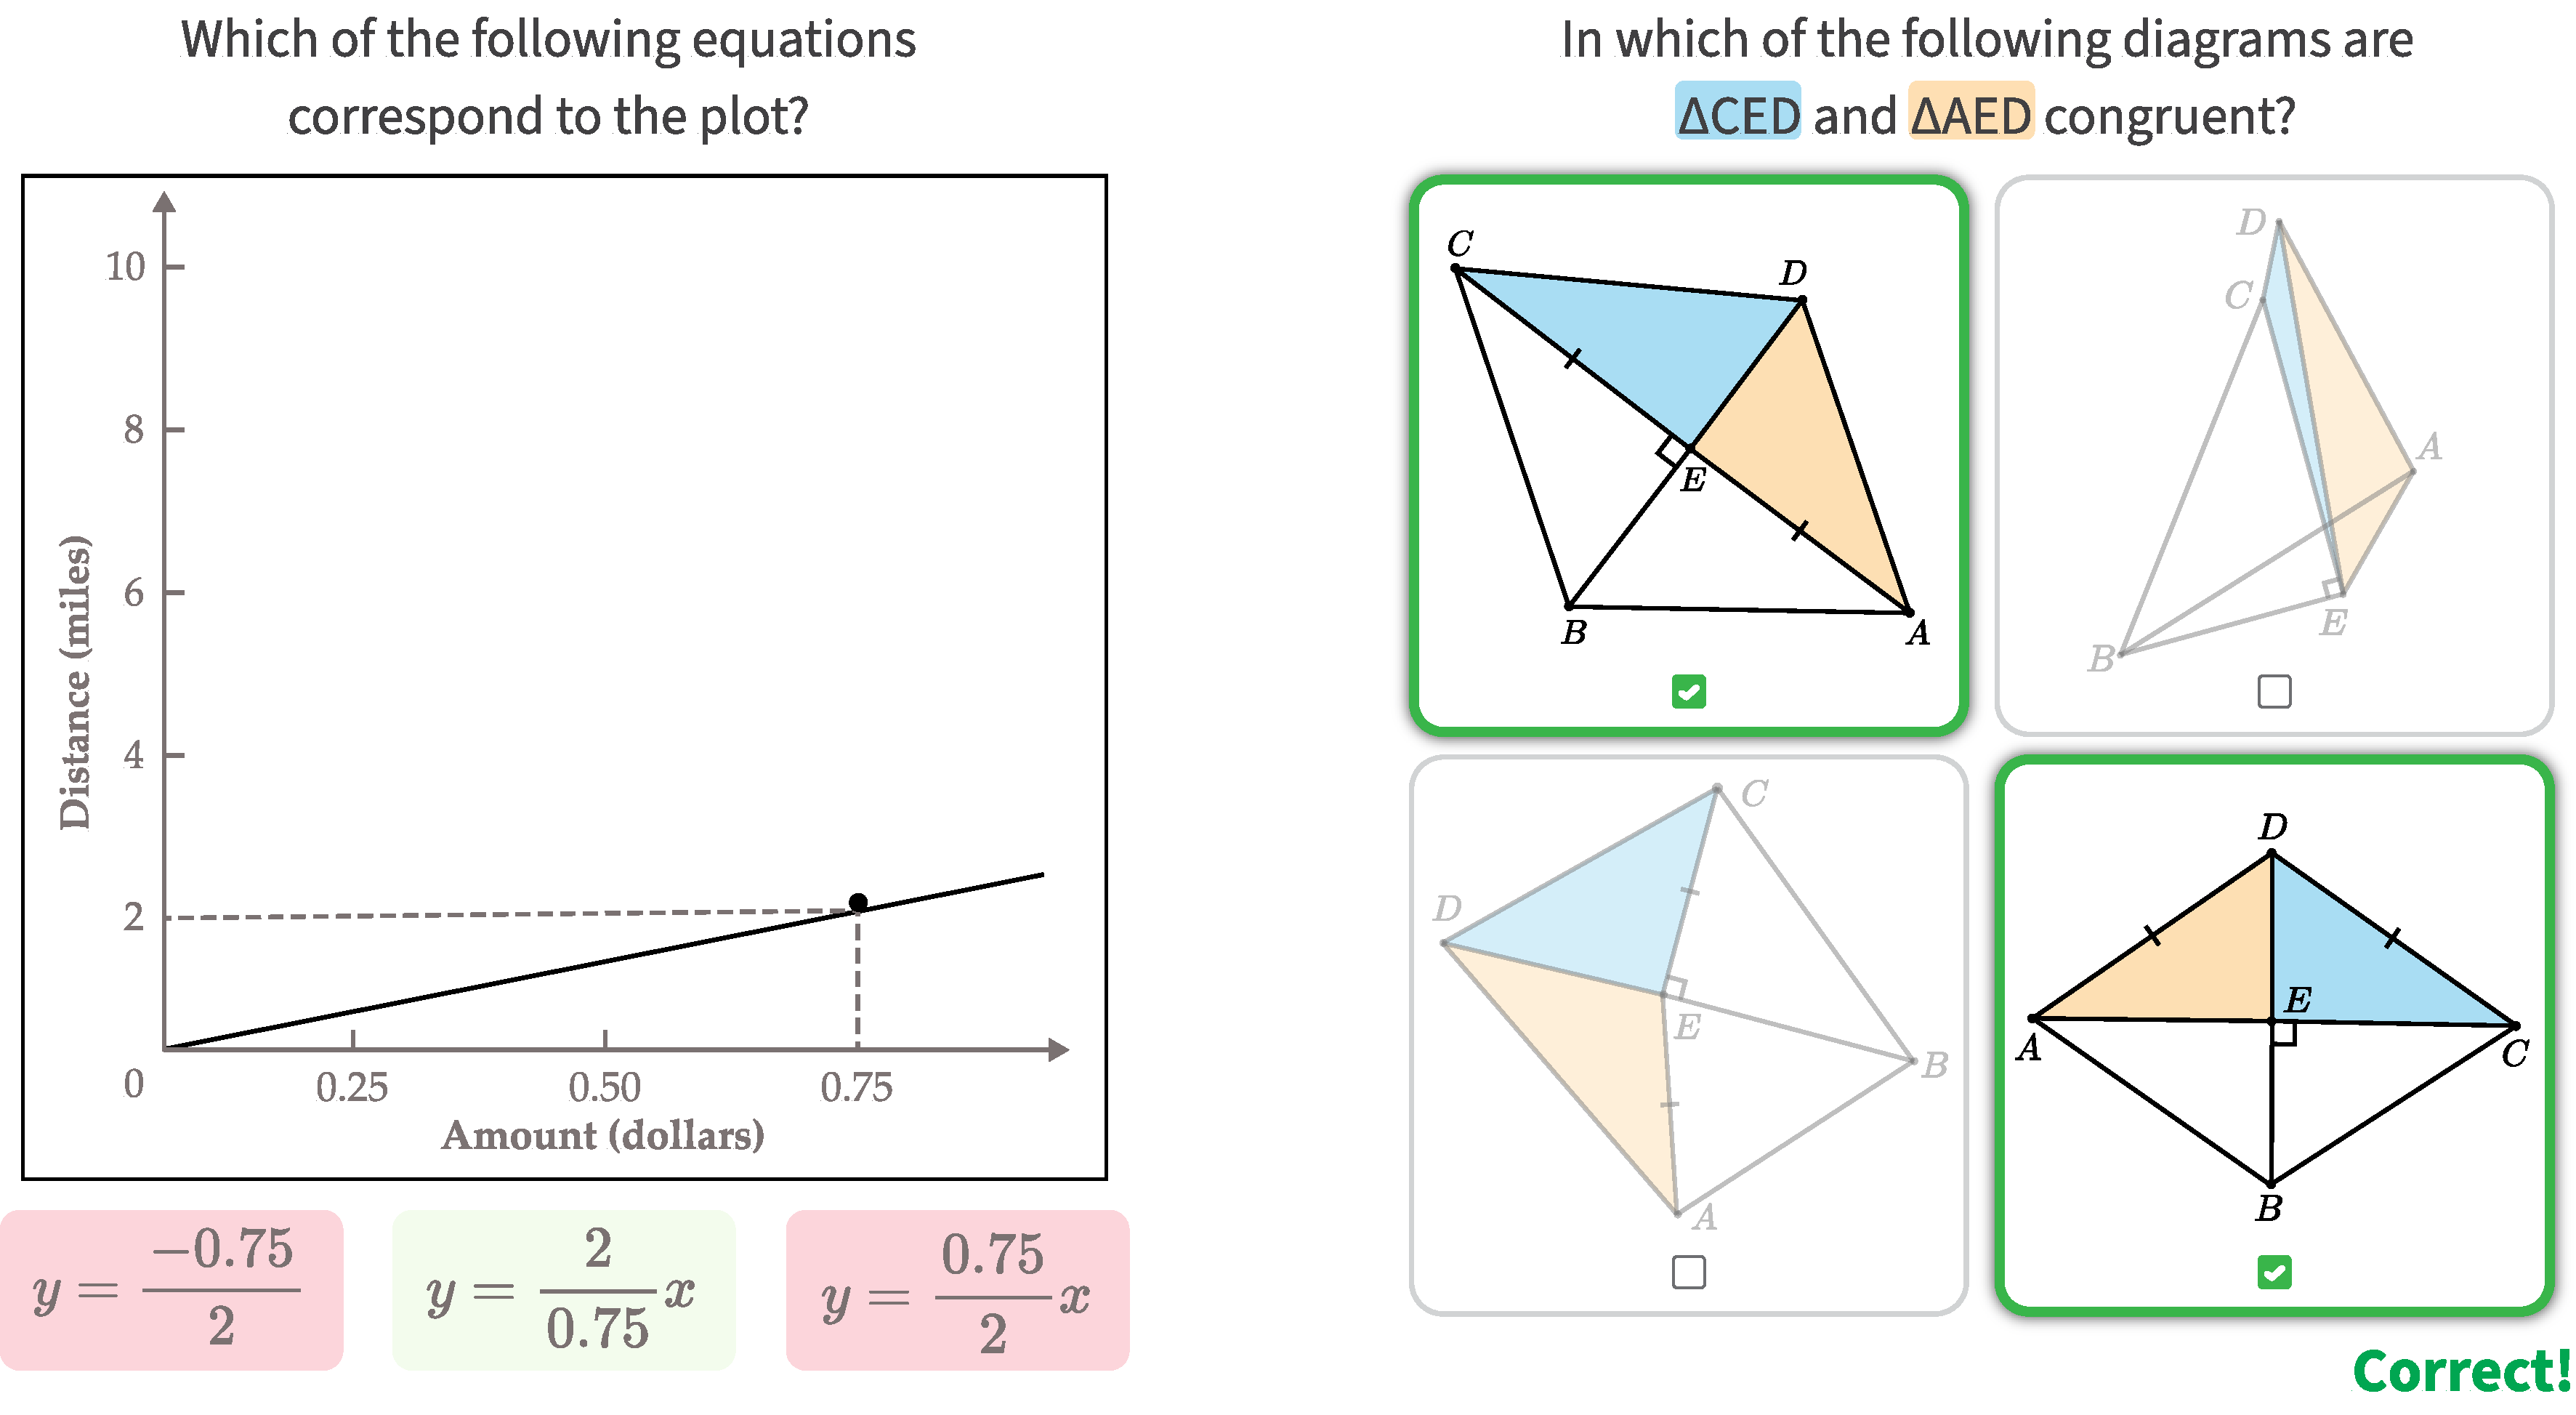
\includegraphics[width=0.88\linewidth]{assets/chapter-3/translation-problem.pdf}
    \caption{\textbf{left}: a translation problem that helps students discern the structure of linear equations (adapted from~\cite{perceptualLearning}). \textbf{right}: an \Edgeworth generated problem that trains student to recognize diagram configurations~\cite{Koedinger1990a} for triangle congruence.}
    \label{fig:translation-problem}
\end{figure}

\vspace{10pt}

\begin{figure}
    \centering
    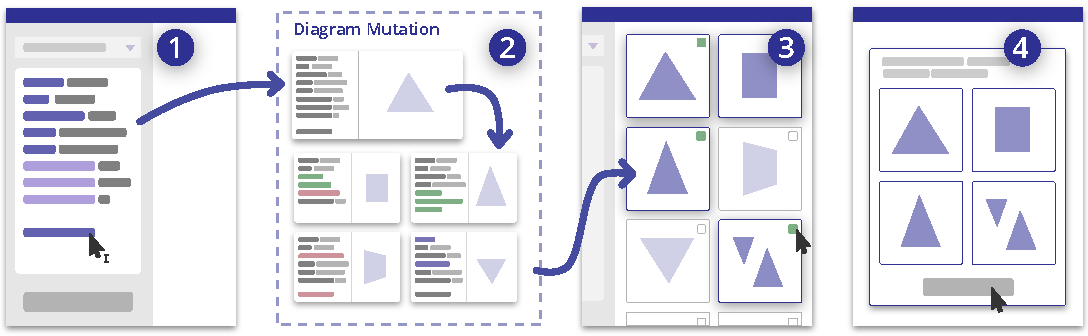
\includegraphics[width=\linewidth]{assets/chapter-3/edgeworth-teaser.pdf}
    \caption{\Edgeworth is a diagrammatic problem authoring tool that automatically generates diagram variations from a single diagram: \textmd{the author creates an example diagram~(\uilabel{1}), then \Edgeworth generates a myriad of diagram variations~(\uilabel{2}), from which the author selects diagrams~(\uilabel{3}) to form a diagrammatic multiple choice problem~(\uilabel{4}).}}
    \label{fig:teaser}
\end{figure}

Effective use of visual representations requires a certain level of \emph{representational fluency} that's achievable through deliberate practice and repetition~\cite{metarepresentation, representationalFluency}. Recognizing how words, symbols, and diagrams relate to each other is an important first step of achieving fluency. Prior work has shown that these contrasting cases, \ie, discrimination and mapping, among representations significantly improve students' ability to translate among representations~\cite{perceptualLearning}.

To train students' representational fluency, educators often create problem sets that involve numerous contrasting cases of a particular visual representation. For instance, \cref{fig:translation-problem}~shows two examples of \emph{translation problems}, where the problem asks students to determine diagrammatic \emph{instances} and \emph{noninstances} of a textual description and vice versa. Importantly, these instances and noninstances have varying degrees of differences from the given diagram or text, and carefully picking examples on this spectrum has a big impact on learning~\cite{samenessAndDifference}.

Traditionally, educators author visual practice by drawing diagrams by hand. In formative interviews (\cref{sec:edgeworth-formative}), educators reported the vital role of visual practice in their instruction, but noted the tedium of authoring due to tool limitations, leading to fewer diagrams used than desired. Manual authoring can hardly keep up with the growth of STEM learners and demand for more visual practice.

As a first step towards scaling up visual practice authoring, we built \Edgeworth, a diagrammatic problem generator. \Edgeworth generates \emph{translation problems}, an effective type of visual practice~\cite{perceptualLearning} that ask students to determine diagrammatic \emph{examples} and \emph{counterexamples} of a textual/symbolic description (\cref{fig:translation-problem}). To help authors get the most out of one diagram, \Edgeworth contributes a ``build once, generate many'' authoring paradigm: Instead of manually editing diagrams to get variations, the author creates a single diagram and \Edgeworth automatically generates diagram variations (\cref{fig:teaser}\uilabel{1}\uilabel{2}). The interaction design of \Edgeworth allows the author to visually select diagram variations to rapidly form translation problems (\cref{fig:teaser}\uilabel{3}\uilabel{4}). Given the diversity of instructional contexts in STEM, we designed \Edgeworth to be domain-agnostic: it uses a generic program mutation technique~(\cref{sec:edgeworth-mutation}) to change the author-provided diagram to produce variations. 

In this chapter, we discuss formative interviews that drove the design of \Edgeworth{} and then walk through the technical implementation of \Edgeworth.

\section{Formative interview}

\label{sec:edgeworth-formative}

We conducted semi-structured interviews with 6 educators to understand how they author, use, and maintain diagrammatic problems. We recruited participants based on their background in education and usage of diagrams in their work. Selected participants work as secondary school teachers, university professors, teaching assistants, and competitive math coaches. All participants (P1--6) indicated that they have experience creating instructional material, authoring problems, and/or developing online courses that include visual content. Example interview questions include what roles diagrams play in the participant's educational materials, how students interact with diagrams, and how diagrams are authored and maintained. The full interview protocol is included in supporting files.

Participants reported the usage of diagrams to build conceptual understanding and emphasized the need for deliberate practice to acquire representational fluency. Traditional educational materials, especially in higher education, tend to emphasize \quotei{procedures, memorization, and symbolic manipulation} (P6).  Similarly, teachers such as P1 suffer from \quotei{the curse of knowledge} of teaching visual fluency: teachers tend to \quotei{under-train} students and they struggle to use visuals for problem-solving.  As a result, students often become \quotei{symbolically good} and do not develop \quotei{good conceptual understanding} (P3). Visuals like diagrams and graphs provide alternative representations that help students \quotei{develop intuition} (P3) and \quotei{become better problem-solvers} (P4). To improve their instruction, all of our participants (P1--6) attempt to incorporate more diagrams in their instructional materials. Some also ask students to draw, annotate, and explain diagrams (P1, P2, P6). P2 encourages students to learn \quotei{multiple representations} and makes diagrams central to their math and programming curricula. When students practice with diagrams, teachers also gain richer feedback on students' level of understanding, and \quotei{learned more from this [student-drawn diagram] than 10 similar problems without the pictures} (P6).

While the benefits of and need for diagrammatic practice are clear, participants reported that tool limitations led to manual and repetitive authoring experience. Because participants typically create many problems and iterate on their content often, they face a trade-off when authoring visual content: more visuals are beneficial for learning but are time-consuming to create and modify. When authoring practice problems, P1 struggled to \quotei{create simple shapes by myself} and always ended up \quotei{copy-pasting and searching online} repeatedly. Similarly, P6 reported that they \quotei{get online images for pre-made resources, but whenever I want something a little custom, it’ll take a lot of time.} To streamline the visual authoring process, P2 and P5 developed custom pipelines for authoring problem sets and quizzes using existing programming tools. Like the problems described by prior research on diagramming tool usability~\cite{naturalDiagramming}, these tools often lack support for \quotei{high-level tweaking of my diagrams} (P2) and \quotei{are a pain to use because the language is not semantic and hard to use for non-programmers} (P5). Participants showed us many examples of tedious changes necessary to create diagram variations.

From the results, we derived the following design requirements for tool design to address participants' needs:

\begin{enumerate}[label=\textbf{D\arabic*}]
    \item\label{req:fluency} Address the need for practicing representational fluency
    \item\label{req:variation} Simplify the workflow for generating diagram variations
    \item\label{req:layout} Obviate the need to attend to low-level diagramming details
\end{enumerate}



\section{System Design of \Edgeworth}
\label{sec:system-design}


\Edgeworth realizes the design goals from \cref{sec:edgeworth-formative} by: 1) providing a domain-agnostic workflow for rapidly authoring diagrammatic practice problems (\ref{req:fluency}), 2) automatically suggesting numerous diagram variations of a single example diagram and allowing the author to visually select from the variations (\ref{req:variation}), and 3) fully automating the layout for all diagram variations (\ref{req:layout}). \cref{fig:edgeworth-interface} walks through the user interface of \Edgeworth, a simple and clean design that encapsulates the ideas above.

In \cref{sec:edgeworth-workflow}, we demonstrate the workflow of \Edgeworth by showing how to author an example diagrammatic problem in Euclidean geometry. We then describe \Edgeworth's approach to diagram layout in \cref{sec:edgeworth-layout} and how it generates diagram variation in \cref{sec:edgeworth-mutation}. 

% Finally, we discuss the limitations of the current implementation in \cref{sec:limitations}.

\begin{figure}
    \centering
    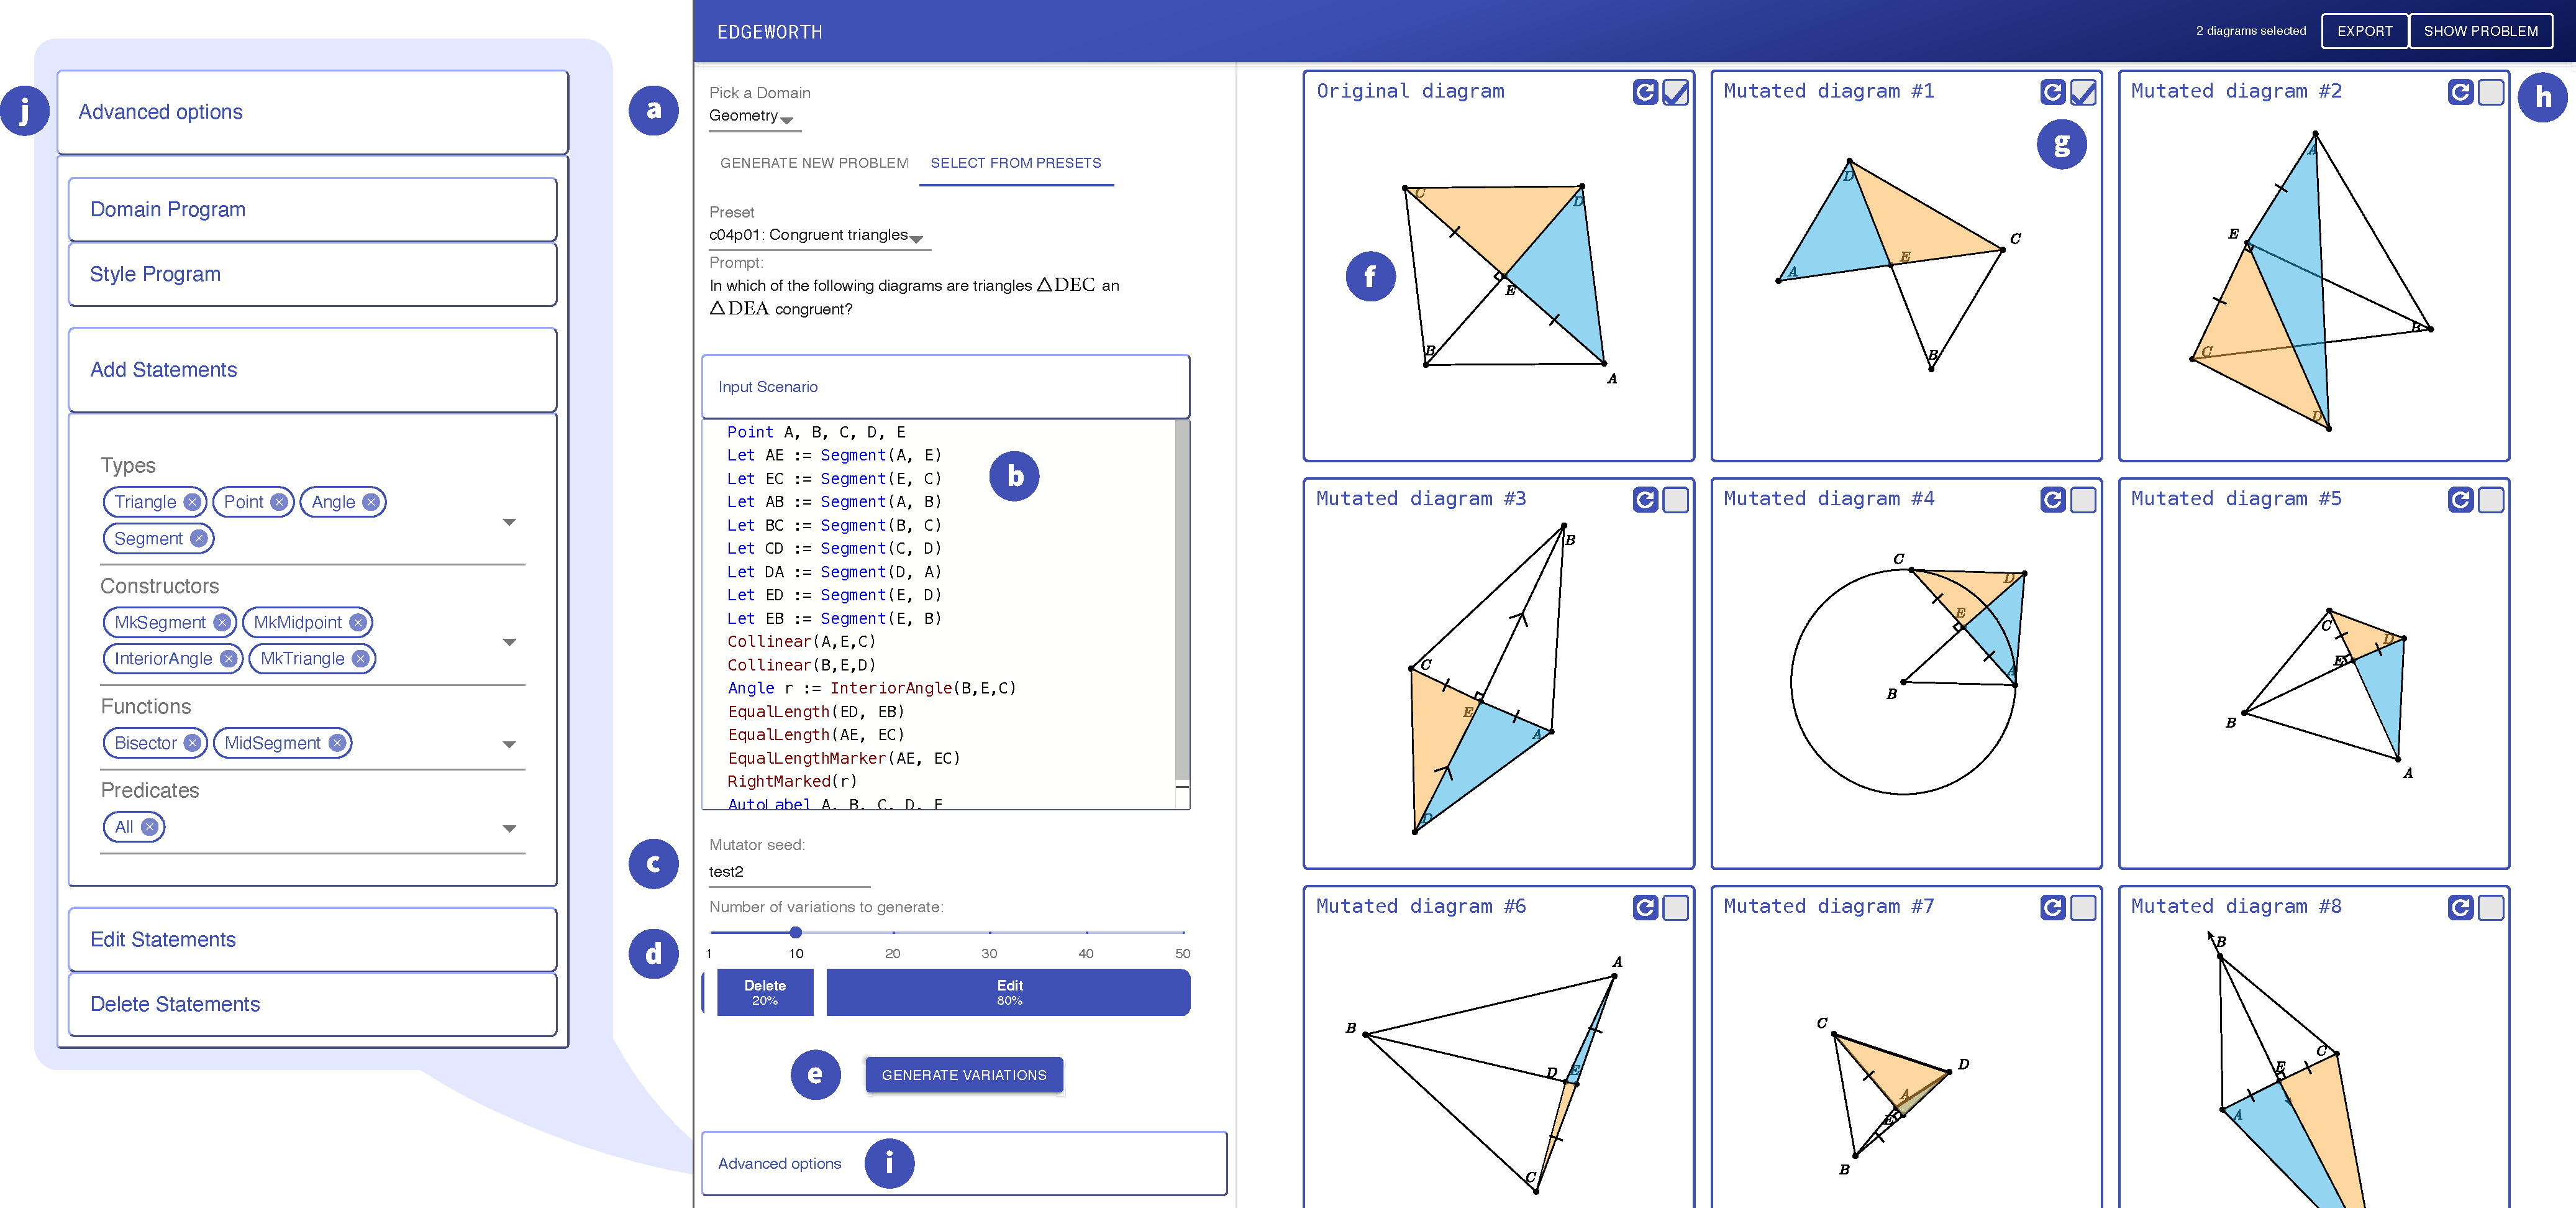
\includegraphics[width=\linewidth]{assets/chapter-3/edgeworth-ui-new.pdf}
    \caption{\textbf{The user interface of \Edgeworth.} \textmd{The author first provides a textual prompt~(\uilabel{a}) as an input scenario in \Substance notation~(\uilabel{b}). Then, clicking ``Generate Variations''~(\uilabel{e}) generates the specified number of diagram variations~(\uilabel{d}) at random based on a string seed and \hl{weights on Add, Delete or Edit mutations}~(\uilabel{c}). In the diagram panel, the top-left diagram~(\uilabel{f}) corresponds to the input scenario and the rest are diagram variations generated by \Edgeworth. The author can visually select diagrams~(\uilabel{g}) to assemble a diagrammatic multiple-choice problem~(\uilabel{h}). If needed, the author can fine-tune the mutator using ``Advanced options'' (\uilabel{i}\uilabel{j}}). }
    \label{fig:edgeworth-interface}
\end{figure}

\subsection{Author Workflow}
\label{sec:edgeworth-workflow}

In this section, we use an example from high school geometry to demonstrate the process of creating a problem in \Edgeworth. 

\subsubsection{Create an example diagram} 
\label{sec:create-scenario}

The author wants to write a problem about triangle congruence to assess students' understanding of the \textit{Side-Angle-Side} (SAS) rule. They want to create a translation problem including one diagram where the SAS rule is satisfied and three others where it is not. The author first describes an example diagram (\cref{fig:edgeworth-interface}\uilabel{b}) where this rule is satisfied. They construct a scenario involving two triangles: $\triangle DEC$ and $\triangle DEA$ share one side $DE$ and have two equal sides $EC$ and $EA$. $\angle CEB$ indicates that $AC$ and $BD$ are perpendicular and therefore $\angle DEC = \angle DEA$. Therefore, $\triangle DEC$ and $\triangle DEA$ are congruent by the SAS rule. Given this description, \Edgeworth lays out the diagram automatically (\cref{fig:edgeworth-interface}\uilabel{f}). 

% \Edgeworth mutates this scenario to create variations that may or may not satisfy the SAS rule, and the author can select from these variations to create their translation problem. While \Edgeworth requires an example scenario, it does not require it to be correct or incorrect. The choice of this scenario is specific to the format of translation problems in this problem set. Constructing the example first guarantees that there will be at least one correct choice in the problem. If the author starts with an incorrect scenario, \Edgeworth may still mutate it to create a correct choice, but it is not guaranteed.

\subsubsection{Select from \Edgeworth-generated diagrams}
\label{sec:select-diagrams}

Now the author can use \Edgeworth to mutate the example diagram by clicking ``Generate Variations'' (\cref{fig:edgeworth-interface}\uilabel{e}). \Edgeworth performs mutations on the example scenario and generates a grid of diagram variations. The grid is designed to give the author an overview of the mutation results, and diagrams are prominent in each cell to facilitate faster visual selection. The top-left cell in the grid will always display the original example diagram (\cref{fig:edgeworth-interface}\uilabel{b}\uilabel{f}), and the rest correspond to mutation results.

By inspecting each diagram in the grid, the author can determine if it is a good fit for their translation problem. If so, they click the top-right checkbox (\cref{fig:edgeworth-interface}\uilabel{g}) to include the diagram in the problem.

\subsubsection{Preview and export the problem}
After the author picks a sufficient number of diagrams (4 in this case), they can preview the translation problem by clicking ``Show Problem'' (\cref{fig:edgeworth-interface}\uilabel{h}), which displays an interactive multiple-choice widget. If the author is satisfied, they can click ``Export'' to download the diagrams and metadata to use the problem in their context. \Edgeworth exports to Scalable Vector Graphics (SVG) images for static media, source programs for interactive use, and detailed mutation trace metadata for comprehensive analysis and reference purposes.

\subsection{Diagram Notation and Layout}
\label{sec:edgeworth-layout}

\Edgeworth is built on \Penrose~\cref{chp:penrose}. Compared with alternatives, \Penrose offers two advantages: (1) a high-level diagram notation that's easy for authoring and (2) an automatic layout engine. A diagram in \Penrose consists of a textual description of the diagram content (\Substance) and a reusable layout stylesheet. 

\Substance is a simple declarative notation for describing objects and relations in a diagram. As shown in \cref{fig:cocl2-example}, \Substance has three kinds of statements: type statements (\eg \sub{Carbon c}) declare new objects; constructors (\sub{Bond b1 := MakeSingleBond(c, cl1)}) create new objects from existing objects; and predicates (\sub{ZeroValenceElectrons(c)}) indicate relations among objects. A stylesheet translates the \Substance notation to shapes and layout constraints, and then \Penrose solves for diagram layouts automatically. Since \Edgeworth authors only interact with \Substance, we omit the description of the stylesheet language in this paper; more details about stylesheets can be found in the official documentation\footnote{\url{https://penrose.cs.cmu.edu/docs}} and \citet{penrose}.

% \begin{wrapfigure}{r}{0.5\textwidth}
\begin{figure}[H]
    % \begin{center}
    \centering
    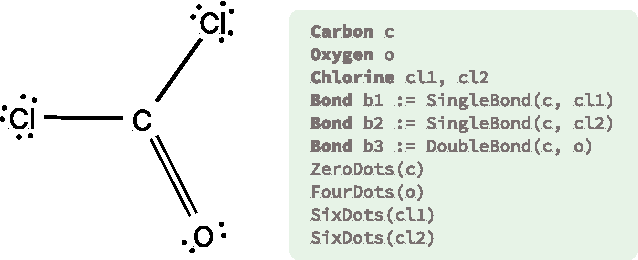
\includegraphics[width=.6\linewidth]{assets/chapter-3/cocl2-example.pdf}
    % \end{center}
    \caption{\textmd{Diagram and \Substance notation for the Lewis structure of phosgene (\ensuremath{\mathrm{COCl_2}}).}}
    \label{fig:cocl2-example}
\end{figure}

The \Penrose ecosystem offers a wide range of stylesheets for STEM diagrams, and the current \Edgeworth implementation builds on \Penrose's geometry, chemistry, and graph stylesheets for diagram layout. Since the existing \Penrose stylesheets are primarily used to generate a few human-written examples, they lack coverage for variations of \Substance descriptions required by \Edgeworth. To this end, we improved stylesheets, diagram examples, and new standard library functions to \Penrose.

\Edgeworth is the first application of \Penrose that concurrently optimizes and renders a grid of multiple diagrams. Therefore, we have made significant updates to \Penrose to support \Edgeworth's use case. To make \Edgeworth a performant client-side web application for interactive use, we have migrated from Haskell to TypeScript and made various performance improvements to efficiently run tens of layout optimization jobs in a single session. Compared to the state of \Penrose at the publication of \citet{penrose}, the development of \Edgeworth has helped improve the performance of the system by 100$\times$.


\subsection{Program Mutation}
\label{sec:edgeworth-mutation}

% what is program mutation and why it's a good fit
\Edgeworth generates diagram variations by mutating the example diagram written in \Substance. 
% what the operators are
We purposely designed the system to include a small set of simple and type-safe mutation operations. Similar to generic tree-editing algorithms~\cite{gumtree}, \Edgeworth supports 3 kinds of mutation operators: \textbf{Add}, \textbf{Delete}, and \textbf{Edit}. \textbf{Add} appends a statement. \textbf{Delete} removes a statement and all other references to that statement. 

Since compilation errors in \Substance will not produce diagrams, \textbf{Edit} involves one of the type-safe patterns listed below. Each \textbf{Edit} pattern contains a \emph{guard} and an \emph{action}. The guard checks if the operator is applicable to the given \Substance statement, and the action performs the mutation. For instance, \textbf{Replace Arguments} is only applicable when the current context has existing variables of the desired type. 
\begin{itemize}[leftmargin=*]
    \item \textbf{Swap Arguments} reorders the arguments passed into a statement; \eg if \sub{A} and \sub{B} are \sub{Triangle}s:\\
            \sub{Similar(A, B)} $\rightarrow$ \sub{Similar(B, A)}
    \item \textbf{Replace Arguments} replaces the arguments passed into a statement with other arguments defined in scope; \eg if \sub{A, B, C, D} are \sub{Point}s:\\
            \sub{s := MkSegment(A, B)} 	$\rightarrow$ \sub{s := MkSegment(C, D)}
    \item \textbf{Replace Function} replaces a statement with a different statement that takes the same arguments; \eg if \sub{T} is a \sub{Triangle} and \sub{E} is an \sub{Angle}:\\
            \sub{Equilateral(T)} $\rightarrow$ \sub{Scalene(T)} \\
            \sub{Segment s := Bisector(E)} $\rightarrow$ \sub{RightAngleMarked(E)}
\end{itemize}

% one-col
\begin{algorithm}
\caption{The \Edgeworth mutation algorithm. }\label{alg:mutation}
\begin{algorithmic}[1]
\Function{Generate}{$p, \ell, h, a, d, e, A, D, E$}
\State $p' \gets p$
\State $n \gets \text{uniform random integer between $\ell$ and $h$}$\label{line:mutations}
\For{$i$ \textbf{from} $1$ \textbf{to} $n$}
    \State $x \gets \text{uniform random real between $0$ and $a + d + e$}$\label{line:kind}
    \If{$x < a$}
        \State $m \gets \textsc{RandomAdd}(A, p')$\label{line:add}
    \ElsIf{$x < a + d$}
        \State $m \gets \textsc{RandomDelete}(D, p')$\label{line:delete}
    \Else
        \State{$s \gets \text{uniform random element of $\textsc{Statements}(p')$}$}\label{line:statements}
        \State{$m \gets \textsc{RandomEdit}(E, s)$}\label{line:edit}
    \EndIf
    \State $p' \gets \textsc{Mutate}(p', m)$
\EndFor
\State \textbf{return} $p'$
\EndFunction
\end{algorithmic}
\end{algorithm}
% one-col

Algorithm~\ref{alg:mutation} shows how the \Edgeworth mutator works, at a high level. In addition to the input \Substance description $p$, \Edgeworth also takes a number of user-defined configuration parameters: (1) a number of variations to generate (the number of times \textsc{Generate} is called); (2) a range of mutation counts per variation (the input variables $\ell$ and $h$); (3) weights for \textbf{Add}, \textbf{Delete}, and \textbf{Edit} operations (the input variables $a$, $d$, and $e$ respectively); and (4) filter sets $A$, $D$, and $E$ which limit the set of mutations that the \textbf{Add}, \textbf{Delete}, and \textbf{Edit} operations can produce.

% how the mutator produces mutants
Given an example diagram, \Edgeworth performs several rounds of mutation generation. Each round results in a series of mutations that alter the input to produce a variation. The number of mutations (line~\ref{line:mutations}) is bounded by the configuration parameters.

To generate a single mutation, \Edgeworth makes a weighted choice (line~\ref{line:kind}) of the mutation kinds and enumerates all possible mutations for the chosen kind: \textbf{Add} enumerates all possible statements to add (line~\ref{line:add}); \textbf{Delete} randomly deletes an existing statement (line~\ref{line:delete}); \textbf{Edit} enumerates all possible edits for all statements (line~\ref{line:statements}) and picks one of them randomly (line~\ref{line:edit}). The randomness of \Edgeworth is controlled by a single random generator seed.

Users can specify filter sets under the ``Advanced options'' section of the UI, shown in \cref{fig:edgeworth-interface}\uilabel{i}\uilabel{j}. The filters default to ``All,'' which indicates that the mutator may change any statement in the example diagram. While this precise configuration may be useful, we ended up not using them in our evaluation (\cref{chp:edgeworth-eval}) and instead achieving our results using only \Edgeworth's simpler core set of configuration options, i.e., weights on mutation operators.

% \section{Mutation-based diagram generation}
% \label{sec:edgeworth-mutation}

% Educators simply don't have enough time to produce good-looking diagrams, not to mention the amount and variety of diagrams required for training students to be fluent in visual representations. Therefore, a key pain point to automate is diagram generation. Importantly, the generated diagrams have to be meaningful and need to include contrasting cases of the same subject matter. 

% In \Edgeworth, I propose to \textbf{generate a large pool of diagrams by mutating the \Substance program in a \Penrose trio}. Compared with general-purpose programming languages, \Penrose DSLs have unique advantages: \Domain is a meta-language that precisely defines the available program constructs in \Substance, which helps define the mutation search space. Moreover, it’s easier to make sense of mutation on \Substance, because it corresponds to the domain-specific vocabulary of diagram authors. 

% At a high level, the \Edgeworth mutator takes in a \Penrose trio and a small configuration file, and simply generates an arbitrary number of \Substance programs. Constrained by the configuration, \Edgeworth mutates the \Substance program (\emph{prompt program}) by applying a series of program mutations to get a \emph{mutant} \Substance program. For each mutant, the system then uses the original \Style and \Domain programs to render a diagram. 
 
% \begin{figure}[h]
%     \centering
%     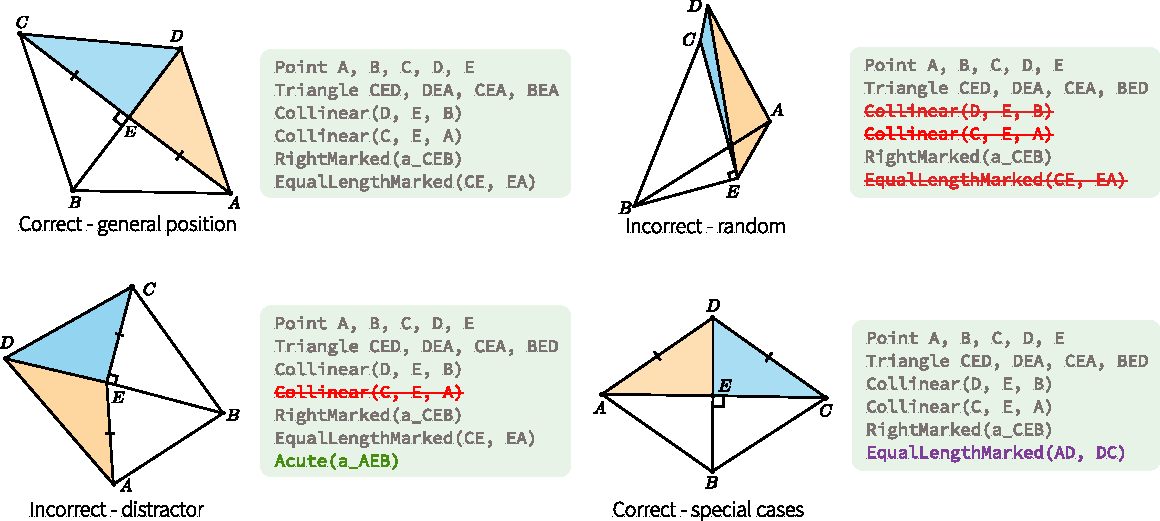
\includegraphics[width=\linewidth]{assets/chapter-3/answer-types.pdf}
%     \caption{Four example classes of mutants generated by \Edgeworth. \textbf{Top-left}: the original prompt program, representing a general correct instance. \textbf{Bottom-Left}: an incorrect noninstance that only slightly differs from the original prompt semantically. \textbf{Top-right}: an incorrect noninstance that differs significantly from the prompt. \textbf{Bottom-right}: a correct instance that's a corner-case of the prompt.}
%     \label{fig:answer-types}
% \end{figure}

% Since \Substance is a small declarative language, \Edgeworth uses a set of pre-defined, high-level mutation operations listed below. 

% \begin{itemize}
%     \item \textbf{Add} Appends a statement to the \Substance program.
%     \item \textbf{Delete} Removes a random statement from the \Substance program.
%     \item \textbf{Cascading Delete} Removes a random statement and all other references to that statement.
%     \item \textbf{Swap Arguments} Reorders the arguments passed into a statement. \eg, if \sub{A} and \sub{B} are \sub{Triangles}:
    
%             \sub{Similar(A, B)} $\rightarrow$ \sub{Similar(B, A)}
%     \item \textbf{Swap-In Arguments} Replaces the arguments passed into a statement with other arguments defined in scope. \eg, if \sub{A, B, C, D} are \sub{Points}:
            
%             \sub{s := MkSegment(A, B)} 	$\rightarrow$ \sub{s := MkSegment(C, D)}
%     \item \textbf{Replace Statement Name} Replaces a statement with a different statement that takes the same type of arguments and has the same return type. \eg, given that \sub{T} is a \sub{Triangle}:
            
%             \sub{Right(T)} $\rightarrow$ \sub{Obtuse(T)}
%     \item \textbf{Type Change} Replaces a statement with a new one that takes the same number and type of arguments, but does not necessarily return a value of the same type. \eg, if \sub{E} is an \sub{Angle}:
            
%             \sub{Segment s := Bisector(E)} $\rightarrow$ \sub{Right(E)}
% \end{itemize}

% These mutations are all done safely at the level of the abstract syntax tree (AST) and \Edgeworth maintains a local context and symbol table, so operations will not introduce errors. The configuration file contains a set of rules to filter down the search space by statement types and specify the kinds of mutations allowed. 

% Authoring contrasting cases require different classes of diagrams: those that correctly correspond to the textual/symbolic description and others that don't. Importantly, nearest neighbors of the prompt program seem to have great education values, \ie, ``near misses'' and ``near hits.'' Knowing the correctness of a mutant also helps with automated grading of problems. 

% Although \Edgeworth generates syntactically valid mutants, the system doesn't know whether a mutant is semantically consistent with the prompt \apriori. Currently, the system uses the graphical constraints to determine semantic consistency. Specifically, it uses an energy-based heuristic by performing \textbf{cross-instance energy evaluation (CIEE)} of each mutant. Suppose \Edgeworth mutates the prompt program $P$ to mutant $P'$ and generates a diagram $D'$ from $P'$. the system can compute the cross-instance energy of $D'$ by 1) checking if all of the constraints generated from $P$ are met by $D'$ and 2) run the objective function defined by $P$ on $D'$ and check if the $D'$ is at a local minimum.  In other words, the \Penrose optimizer determines if the diagram $D'$ generated from mutated program $P'$ is a good fit for the prompt program.

% \vspace{10pt}

% \begin{figure}[h]
%     \centering
%     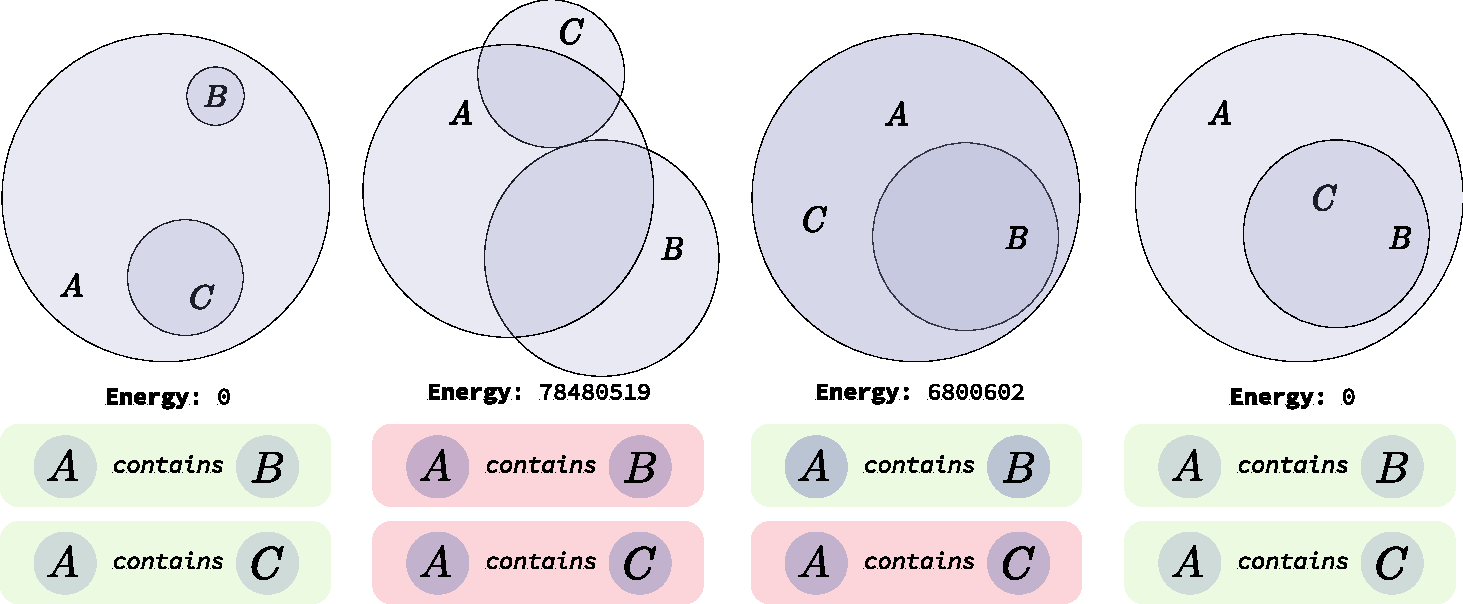
\includegraphics[width=\linewidth]{assets/chapter-3/ciee.pdf}
%     \caption{An example of CIEE, where the leftmost is the prompt program $P$ and its corresponding diagram $D$. The overall energy value is $0$. The right three are instances of $P'$, on which the constraints from the prompt are evaluated. The middle two are \textit{semantically inconsistent} with the prompt and have high energy values. The rightmost is \textit{semantically consistent} with the prompt and therefore has an energy value of $0$.}
%     \label{fig:ciee}
% \end{figure}

% \vspace{10pt}

% \begin{proposed}
% \textbf{CIEE robustness.} CIEE showed some promise on a limited set of examples, but further evaluation is needed to see the robustness of this heuristic. For instance, how much does this method depend on the qualities of the \Style program that defined the constraints? If the mutant significantly differs from the prompt (\eg, missing most identifiers from the prompt), is this heuristic still useful?

% \textbf{\Domain language extensions.} None of the predefined mutations listed above carry any mathematical semantics because \Domain doesn't contain enough information. For instance, many mathematical predicates have reflexive, symmetric, transitive, and substitution properties, but \Domain only encodes basic type definitions. For a more precise notion of correctness, I plan to extend \Domain to model such properties, and use them in the \Edgeworth mutator, possibly together with CIEE, to generate higher quality mutants.  

% \end{proposed}

% \section{Preliminary evaluation of the \Edgeworth mutator}
% \label{sec:edgeworth-prelim-eval}

% In preliminary work, we evaluated the system by recreating problems in a middle-school geometry textbook \cite{holtGeometry}. We examined all 53 diagrammatic problems in the chapter review sections and picked a representative subset of 24 problems and implemented them in \Edgeworth. For each textbook problem, the prompt is reframed so that the diagram accompanying the original problem can be considered a correct answer. Then, we consider possible answers to the posed question, including ``distractors''---answers that are designed to tempt students with limited conceptual understanding---as well as correct ``special cases''. We then describe the original diagram as a prompt \Substance program and pass it to \Edgeworth, which generates numerous answers to the original problem.

% We examined sets of 20 diagrams generated by \Edgeworth based on various prompt programs. Each program was mutated 1-3 times and the correctness of each diagram was determined manually. We found that while \Edgeworth easily generates a variety of correct and incorrect diagrams, careful selection of configuration parameters was often required to get more ``interesting'' diagrams (correct special cases, distractors).

% \begin{proposed}
% \label{prop:config-usability}
% \textbf{Usability of the \Edgeworth configuration.} As noted above, results from the \Edgeworth mutator are sensitive to the configuration. For instance, a statement in the \Substance program might be particularly more suitable for mutations than others (perhaps because it contributes to the correctness of the problem.) Under- or over-specifying mutations in the configuration might lead to a pool of ``noisy'' diagrams. I propose to conduct a light-weight case study with a handful of problems to identify the key to successful configurations. With that insight, we can either improve the configuration format or explore other modes of interaction.
% \end{proposed}

% \section{Mutation paths as problem templates}
% \label{sec:edgeworth-mutation-paths}

% \begin{proposed}
% After generating a pool of diagrams, the author then picks a subset of them for a single \emph{problem instance}. For each generated diagram, \Edgeworth keeps a record of the series of mutations performed on the prompt program (\emph{mutation path}) to the mutant. For a multiple choice problem with four options, there will be four mutation paths from the prompt. Together these paths form a \emph{problem template}.

% A problem template is specific to a prompt, so it's unlikely to be reusable for generating other problem instances. However, many problems might share the same instructional goal such as teaching students the conditions for the Hypotenuse-Leg (HL) theorem. While the choice of names and diagram design may differ, the core structure is the same: two instances of congruent triangles satisfying HL and two noninstances of non-congruent triangles. Encoding this information can further scale up problem authoring. 

% I propose to \textbf{investigate common structures among problem templates and encode them as problem template specifications that are generalizable to multiple prompts}. 

% \end{proposed}

% \section{By-example workflow for authoring at scale}
% \label{sec:edgeworth-by-example}

% With the \Edgeworth mutator, the primary mode of interaction is picking examples from the mutant pool and editing the configuration to narrow down the search space. In some cases (see \cref{prop:config-usability}), the author might want to write a few examples from scratch, or prefer to manually make slight tweaks to examples in the mutant pool. I propose to \textbf{create a programming-by-example workflow, where the author manually creates a few diagrams and \Edgeworth generates a bigger pool of diagrams with similar properties}.

% \vspace{10pt}
% \begin{figure}[h]
%     \centering
%     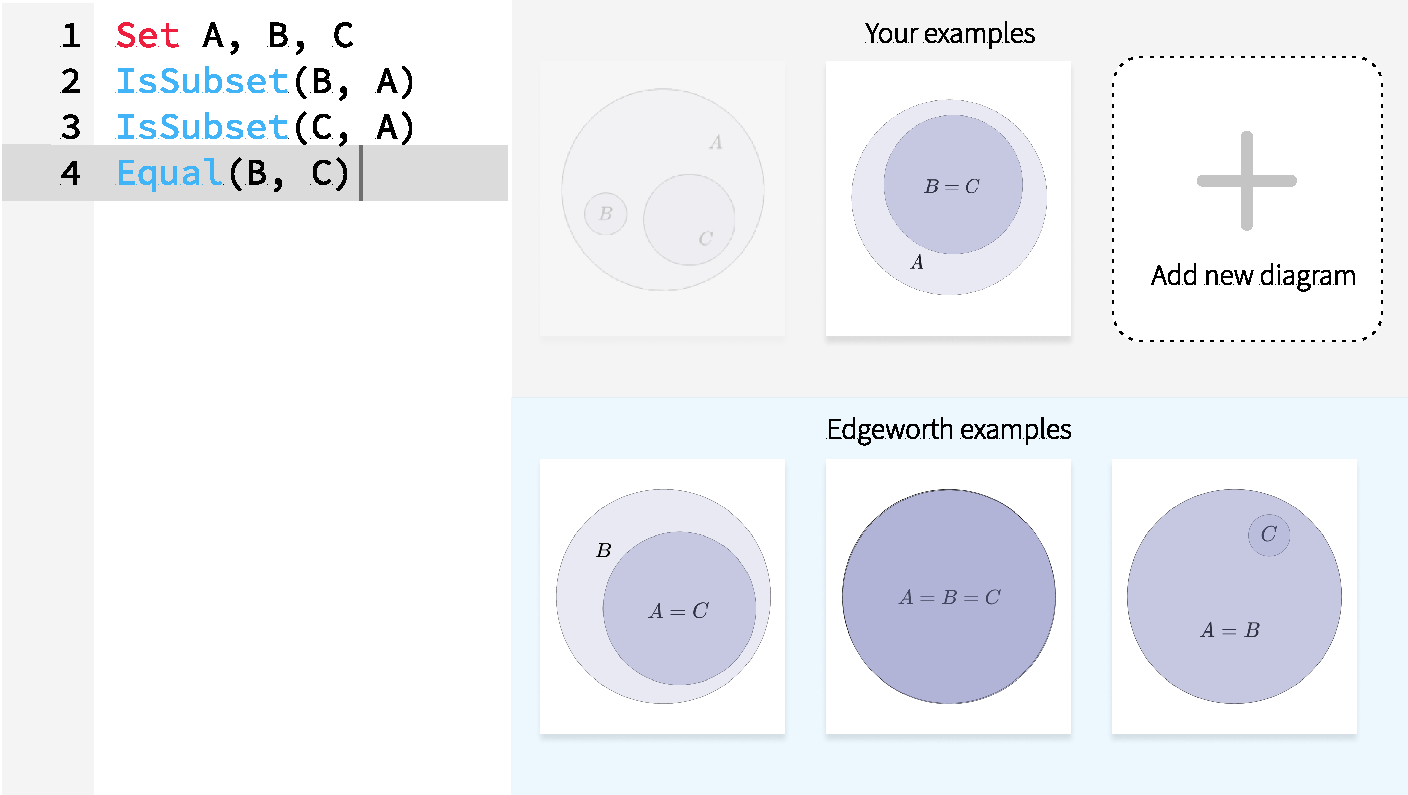
\includegraphics[width=\linewidth]{assets/chapter-3/synthesis-driven-workflow.pdf}
%     \caption{User interface mock-up of a by-example workflow in \Edgeworth.}
%     \label{fig:synthesis-driven-workflow}
% \end{figure}
% \vspace{10pt}

% For example, if \Edgeworth fails to generate a pool of useful diagrams, the author can manually create a few examples by directly editing the prompt program. In \cref{fig:synthesis-driven-workflow}, the author adds the \sub{Equal(B, C)} predicate. Their intent is to include the edge case of proper subsets in this problem, where some of the subset relations are actually equality. \Edgeworth generates a set of similar examples that add \sub{Equal} predicates with existing identifiers in different ways. 

% The addition of \sub{Equal(B, C)} is effectively a user-generated mutation, and \Edgeworth needs to understand this mutation to generate similar instances. Currently, the \Edgeworth synthesizer matches a series of author edits to predefined mutations. Once the synthesizer finds a path, it can then inform the mutator to generate examples with similar properties (\ie, including the edge case of equal sets). 

% \begin{proposed}
% \textbf{Generalized mutation paths} Similar to templates, the by-example workflow also requires a generalizable encoding of mutations. I plan to experiment with a few possible formats such as (1) another mutator configuration and (2) mutation paths with ``holes.''
% \end{proposed}

% \section{Evaluation}

% \begin{proposed}
% \textbf{Usability study of \Edgeworth.} I propose to evaluate the usability of \Edgeworth by recruiting authors to perform content authoring tasks with the \Edgeworth prototype. For example, the participants may be asked to author a problem set of 10 diagrammatic problems. The goal of this study will be to identify missing features, usability problems, and opportunities for simplification. The study may include several rounds with increasingly high-fidelity prototypes. After each round, I will refine the design and implement the next prototype. Here are some possible research questions:
% \begin{itemize}
%     \item  What are the key design considerations for diagrammatic problem authoring? How do they fit with the features of \Edgeworth?
%     \item How do authors prefer to work with \Edgeworth? When do they opt to write a configuration file and generate many diagrams? When do they use the by-example workflow? Do they mix the two workflows?
%     \item How does the experience compare to their existing tools? How can \Edgeworth incorporate useful parts of them? 
% \end{itemize}
% \end{proposed}

